\documentclass{ximera}

\title{Practice for Advanced Nonlinear Analysis}

%\auor{Matthew Charnley and Jason Nowell}
\usepackage[margin=1.5cm]{geometry}
\usepackage{indentfirst}
\usepackage{sagetex}
\usepackage{lipsum}
\usepackage{amsmath}
\usepackage{mathrsfs}


%%% Random packages added without verifying what they are really doing - just to get initial compile to work.
\usepackage{tcolorbox}
\usepackage{hypcap}
\usepackage{booktabs}%% To get \toprule,\midrule,\bottomrule etc.
\usepackage{nicefrac}
\usepackage{caption}
\usepackage{units}

% This is my modified wrapfig that doesn't use intextsep
\usepackage{mywrapfig}
\usepackage{import}



%%% End to random added packages.


\graphicspath{
    {./figures/}
    {./../figures/}
    {./../../figures/}
}
\renewcommand{\log}{\ln}%%%%
\DeclareMathOperator{\arcsec}{arcsec}
%% New commands


%%%%%%%%%%%%%%%%%%%%
% New Conditionals %
%%%%%%%%%%%%%%%%%%%%


% referencing
\makeatletter
    \DeclareRobustCommand{\myvref}[2]{%
      \leavevmode%
      \begingroup
        \let\T@pageref\@pagerefstar
        \hyperref[{#2}]{%
	  #1~\ref*{#2}%
        }%
        \vpageref[\unskip]{#2}%
      \endgroup
    }%

    \DeclareRobustCommand{\myref}[2]{%
      \leavevmode%
      \begingroup
        \let\T@pageref\@pagerefstar
        \hyperref[{#2}]{%
	  #1~\ref*{#2}%
        }%
      \endgroup
    }%
\makeatother

\newcommand{\figurevref}[1]{\myvref{Figure}{#1}}
\newcommand{\figureref}[1]{\myref{Figure}{#1}}
\newcommand{\tablevref}[1]{\myvref{Table}{#1}}
\newcommand{\tableref}[1]{\myref{Table}{#1}}
\newcommand{\chapterref}[1]{\myref{chapter}{#1}}
\newcommand{\Chapterref}[1]{\myref{Chapter}{#1}}
\newcommand{\appendixref}[1]{\myref{appendix}{#1}}
\newcommand{\Appendixref}[1]{\myref{Appendix}{#1}}
\newcommand{\sectionref}[1]{\myref{\S}{#1}}
\newcommand{\subsectionref}[1]{\myref{subsection}{#1}}
\newcommand{\subsectionvref}[1]{\myvref{subsection}{#1}}
\newcommand{\exercisevref}[1]{\myvref{Exercise}{#1}}
\newcommand{\exerciseref}[1]{\myref{Exercise}{#1}}
\newcommand{\examplevref}[1]{\myvref{Example}{#1}}
\newcommand{\exampleref}[1]{\myref{Example}{#1}}
\newcommand{\thmvref}[1]{\myvref{Theorem}{#1}}
\newcommand{\thmref}[1]{\myref{Theorem}{#1}}


\renewcommand{\exampleref}[1]{ {\color{red} \bfseries Normally a reference to a previous example goes here.}}
\renewcommand{\figurevref}[1]{ {\color{red} \bfseries Normally a reference to a previous figure goes here.}}
\renewcommand{\tablevref}[1]{ {\color{red} \bfseries Normally a reference to a previous table goes here.}}
\renewcommand{\Appendixref}[1]{ {\color{red} \bfseries Normally a reference to an Appendix goes here.}}
\renewcommand{\exercisevref}[1]{ {\color{red} \bfseries Normally a reference to a previous exercise goes here.}}



\newcommand{\R}{\mathbb{R}}

%% Example Solution Env.
\def\beginSolclaim{\par\addvspace{\medskipamount}\noindent\hbox{\bf Solution:}\hspace{0.5em}\ignorespaces}
\def\endSolclaim{\par\addvspace{-1em}\hfill\rule{1em}{0.4pt}\hspace{-0.4pt}\rule{0.4pt}{1em}\par\addvspace{\medskipamount}}
\newenvironment{exampleSol}[1][]{\beginSolclaim}{\endSolclaim}

%% General figure formating from original book.
\newcommand{\mybeginframe}{%
\begin{tcolorbox}[colback=white,colframe=lightgray,left=5pt,right=5pt]%
}
\newcommand{\myendframe}{%
\end{tcolorbox}%
}

%%% Eventually return and fix this to make matlab code work correctly.
%% Define the matlab environment as another code environment
%\newenvironment{matlab}
%{% Begin Environment Code
%{ \centering \bfseries Matlab Code }
%\begin{code}
%}% End of Begin Environment Code
%{% Start of End Environment Code
%\end{code}
%}% End of End Environment Code


% this one should have a caption, first argument is the size
\newenvironment{mywrapfig}[2][]{
 \wrapfigure[#1]{r}{#2}
 \mybeginframe
 \centering
}{%
 \myendframe
 \endwrapfigure
}

% this one has no caption, first argument is size,
% the second argument is a larger size used for HTML (ignored by latex)
\newenvironment{mywrapfigsimp}[3][]{%
 \wrapfigure[#1]{r}{#2}%
 \centering%
}{%
 \endwrapfigure%
}
\newenvironment{myfig}
    {%
    \begin{figure}[h!t]
        \mybeginframe%
        \centering%
    }
    {%
        \myendframe
    \end{figure}%
    }


% graphics include
\newcommand{\diffyincludegraphics}[3]{\includegraphics[#1]{#3}}
\newcommand{\myincludegraphics}[3]{\includegraphics[#1]{#3}}
\newcommand{\inputpdft}[1]{\subimport*{../figures/}{#1.pdf_t}}


%% Not sure what these even do? They don't seem to actually work... fun!
%\newcommand{\mybxbg}[1]{\tcboxmath[colback=white,colframe=black,boxrule=0.5pt,top=1.5pt,bottom=1.5pt]{#1}}
%\newcommand{\mybxsm}[1]{\tcboxmath[colback=white,colframe=black,boxrule=0.5pt,left=0pt,right=0pt,top=0pt,bottom=0pt]{#1}}
\newcommand{\mybxsm}[1]{#1}
\newcommand{\mybxbg}[1]{#1}

%%% Something about tasks for practice/hw?
\usepackage{tasks}
\usepackage{footnote}
\makesavenoteenv{tasks}


%% For pdf only?
\newcommand{\diffypdfversion}[1]{#1}


%% Kill ``cite'' and go back later to fix it.
\renewcommand{\cite}[1]{}


%% Currently we can't really use index or its derivatives. So we are gonna kill them off.
\renewcommand{\index}[1]{}
\newcommand{\myindex}[1]{#1}







\begin{document}
\begin{abstract}
Why?
\end{abstract}
\maketitle


\begin{exercise}
    Find the implicit equations of the trajectories of the following conservative systems.  
    \begin{itemize}
        \item $x''+ x+x^3 = 0$, $C = \answer{\frac{1}{2}y^2 + \frac{x^4}{4} + \frac{x^2}{2}}$
            \begin{problem}
                There is/are:
                \begin{multipleChoice}
                    \choice[correct]{One critical point.}
                    \choice{More than one critical points.}
                    \choice{No critical points.}
                \end{multipleChoice}
                \begin{problem}
                    Classify the critical point: $\left(\answer{0}, \answer{0}\right)$ is a \wordChoice{\choice[correct]{center}\choice{saddle}}.
                \end{problem}
            \end{problem}
        \item $\theta''+\sin \theta = 0$, $C = \answer{\frac{1}{2}y^2 - \cos(\theta)}$
            \begin{problem}
                There is/are:
                \begin{multipleChoice}
                    \choice{One critical point.}
                    \choice[correct]{More than one critical points.}
                    \choice{No critical points.}
                \end{multipleChoice}
                \begin{problem}
                    Classify the critical points: [Use $n$ for a dummy integer.] $\left(\answer{n\pi}, \answer{0}\right)$ is a \wordChoice{\choice{center}\choice[correct]{saddle}} if $n$ is even, and a \wordChoice{\choice[correct]{center}\choice{saddle}} if $n$ is odd. 
                \end{problem}
            \end{problem}
        \item $z''+ (z-1)(z+1) = 0$, $C = \answer{\frac{1}{2}y^2 + \frac{z^3}{3} - z}$
            \begin{problem}
                There is/are:
                \begin{multipleChoice}
                    \choice{One critical point.}
                    \choice[correct]{More than one critical points.}
                    \choice{No critical points.}
                \end{multipleChoice}
                \begin{problem}
                    Classify the critical points: $\left(\answer{1}, \answer{0}\right)$ is a \wordChoice{\choice[correct]{center}\choice{saddle}}, $\left(\answer{-1}, \answer{0}\right)$ is a \wordChoice{\choice{center}\choice[correct]{saddle}}.
                \end{problem}
            \end{problem}
        \item $x''+ x^2+1 = 0$, $C = \answer{\frac{1}{2}y^2 + \frac{x^3}{3} + x}$
            \begin{problem}
                There is/are:
                \begin{multipleChoice}
                    \choice{One critical point.}
                    \choice{More than one critical points.}
                    \choice[correct]{No critical points.}
                \end{multipleChoice}
            \end{problem}
    \end{itemize}
\end{exercise}
%\comboSol
%{%
%a)~$\frac{1}{2}y^2 + \frac{x^4}{4} + \frac{x^2}{2} = C$. $(0,0)$ is a center. \\
%b)~$\frac{1}{2}y^2 - \cos(\theta) = C$. $(n\pi, 0)$ is a saddle if $n$ is even, and a center if $n$ is odd. \\
%c)~$\frac{1}{2}y^2 + \frac{z^3}{3} - z = C$, $(1,0)$ is a center, $(-1, 0)$ is a saddle. \\
%d)~$\frac{1}{2}y^2 + \frac{x^3}{3} + x = C$, no critical points.
%}

\begin{exercise}%
    Find the implicit equations of the trajectories of the following conservative systems.  Next find their critical points (if any) and classify them.
    \begin{itemize}
        \item $x''+ x^2 = 4$, $C = \answer{\frac{1}{2}y^2 + \frac{1}{3}x^3 -4x}$
            \begin{problem}
                There is/are:
                \begin{multipleChoice}
                    \choice{One critical point.}
                    \choice[correct]{More than one critical points.}
                    \choice{No critical points.}
                \end{multipleChoice}
                \begin{problem}
                    Classify the critical points:   $\left(\answer{-2}, \answer{0}\right)$ is a \wordChoice{\choice{stable}\choice[correct]{unstable}} \wordChoice{\choice{center}\choice[correct]{saddle}}.\\
                                                    $\left(\answer{2}, \answer{0}\right)$ is a \wordChoice{\choice[correct]{stable}\choice{unstable}} \wordChoice{\choice[correct]{center}\choice{saddle}}.\\
                \end{problem}
            \end{problem}
        \item $x''+ e^x = 0$, $C = \answer{\frac{1}{2}y^2 + e^x}$
            \begin{problem}
                There is/are:
                \begin{multipleChoice}
                    \choice{One critical point.}
                    \choice{More than one critical points.}
                    \choice[correct]{No critical points.}
                \end{multipleChoice}
            \end{problem}
        \item $x''+ (x+1)e^x = 0$, $C = \answer{\frac{1}{2}y^2 + xe^x}$
            \begin{problem}
                There is/are:
                \begin{multipleChoice}
                    \choice[correct]{One critical point.}
                    \choice{More than one critical points.}
                    \choice{No critical points.}
                \end{multipleChoice}
                \begin{problem}
                    Classify the critical point: $\left(\answer{-1}, \answer{0}\right)$ is a \wordChoice{\choice[correct]{stable}\choice{unstable}} \wordChoice{\choice[correct]{center}\choice{saddle}}.
                \end{problem}
            \end{problem}
    \end{itemize}
\end{exercise}
%\exsol{%
%a) $\frac{1}{2}y^2 + \frac{1}{3}x^3 -4x = C$, critical points:
%$(-2,0)$, an unstable saddle, and $(2,0)$, a stable center. \quad
%b) $\frac{1}{2}y^2 + e^x = C$, no critical points. \quad
%c) $\frac{1}{2}y^2 + xe^x = C$, critical point at $(-1,0)$ is a stable center.
%}


\begin{exercise}%
    The conservative system $x''+x^3 = 0$ is not almost linear.  Classify its critical point(s) nonetheless.\\
    Critical point at: $\left(\answer{0}, \answer{0}\right)$, with trajectories: $y = \pm \answer{\sqrt{2C-(\frac{1}{2})x^4}}$ [Use $C$ as your arbitrary constant].\\
    The critical point is a \wordChoice{\choice[correct]{stable}\choice{unstable}} \wordChoice{\choice[correct]{center}\choice{saddle}}.
\end{exercise}
%\exsol{%
%Critical point at $(0,0)$.
%Trajectories are $y = \pm \sqrt{2C-(\frac{1}{2})x^4}$, for $C > 0$, these give closed
%curves around the origin, so the critical point is a stable center.
%}

\begin{exercise}
    Determine if the following system is Hamiltonian. 
    \[ 
        \frac{dx}{dt} = x - 2y \qquad \frac{dy}{dt} = 3x - y.
    \]
    \begin{multipleChoice}
        \choice[correct]{It is Hamiltonian}
        \choice{It is not Hamiltonian}
    \end{multipleChoice}
    \begin{problem}
        Find the general solution in the form $H(x,y) = C$ and sketch some of the trajectories. $H(x,y) = \answer{-\frac{3}{2}x^2 + xy - y^2}$
    \end{problem}
\end{exercise}
%\comboSol
%{%
%$H(x,y) = -\frac{3}{2}x^2 + xy - y^2$
%}

\begin{exercise}
    Determine if the following system is Hamiltonian. If it is, find the general solution in the form $H(x,y) = C$ and sketch some of the trajectories.
    \[ 
        \frac{dx}{dt} = 4x - 2y + 2 \qquad \frac{dy}{dt} = -5x + y - 1.
    \]
    \begin{multipleChoice}
        \choice{It is Hamiltonian}
        \choice[correct]{It is not Hamiltonian}
    \end{multipleChoice}
\end{exercise}
%\comboSol
%{%
%No
%}


\begin{exercise}
    Determine if the following system is Hamiltonian. If it is, find the general solution in the form $H(x,y) = C$ and sketch some of the trajectories.
    \[ 
        \frac{dx}{dt} = x^2 - 2xy + 3y^2 \qquad \frac{dy}{dt} = y^2 - 2xy + e^x .
    \]
    \begin{multipleChoice}
        \choice[correct]{It is Hamiltonian}
        \choice{It is not Hamiltonian}
    \end{multipleChoice}
    \begin{problem}
        Find the general solution in the form $H(x,y) = C$ and sketch some of the trajectories. $H(x,y) = \answer{x^2y - xy^2 + y^3 - e^x}$
    \end{problem}
\end{exercise}
%\comboSol
%{%
%$H(x,y) = x^2y - xy^2 + y^3 - e^x$
%}


\begin{exercise}
    Determine if the following system is Hamiltonian. If it is, find the general solution in the form $H(x,y) = C$ and sketch some of the trajectories.
    \[ 
        \frac{dx}{dt} = 3x - 4xy \qquad \frac{dy}{dt} = 5xy - y.
    \]
    \begin{multipleChoice}
        \choice{It is Hamiltonian}
        \choice[correct]{It is not Hamiltonian}
    \end{multipleChoice}
    \begin{problem}
        Afterwards, do the same but with the system 
        \[ 
            \frac{dx}{dt} = \frac{3}{y} - 4 \qquad \frac{dy}{dt} = 5 - \frac{3}{x}, 
        \] 
        noticing that this is the same as the first system with each equation divided by $xy$.
        \begin{multipleChoice}
            \choice[correct]{It is Hamiltonian}
            \choice{It is not Hamiltonian}
        \end{multipleChoice}
        \begin{problem}
            Find the general solution in the form $H(x,y) = C$ and sketch some of the trajectories. $H(x,y) = \answer{3\ln(|y|)  + \ln(|x|) - 5x - 4y}$
        \end{problem}
    \end{problem}
\end{exercise}
%\comboSol
%{%
%First is not Hamiltonian. Second is with $H(x,y) = 3\ln(|y|)  + \ln(|x|) - 5x - 4y$.
%}

\begin{exercise} 
    Consider a generic thing on a spring, with displacement $u$ and velocity $v$. Assume that $$mu''+ku=0,$$ where $m$ and $k$ are some positive constants.
    \begin{itemize}
        \item Rewrite this equation as a {\it first-order} system in $u$ and $v$. $u' = \answer{v}$, $v'= \answer{-\frac{k}{m}u}$
        \item Find a Hamiltonian function for this system (in terms of $u$ and $v$). $\answer{\frac{v^2}{2} + \frac{k}{m}u^2}$
        \item What shapes are the level curves of the Hamiltonian function? 
        \item Does this system have a {\it basin of attraction}? \wordChoice{\choice{Yes.}\choice[correct]{No.}}%Explain briefly. 
    \end{itemize}
\end{exercise}
%\comboSol
%{%
%a)~$u' = v$, $v'= -\frac{k}{m}u$ \quad b)~ $\frac{v^2}{2} + \frac{k}{m}u^2$ \quad c)~ Ellipses \quad d)~ No
%}

\begin{exercise}
    Suppose $f$ is always positive. Find the trajectories of $x''+f(x') = 0$. Are there any critical points?\\
    \wordChoice{\choice{Yes.}\choice[correct]{No.}}
\end{exercise}
%\comboSol
%{%
%No.
%}

\begin{exercise}
    Suppose that $x' = f(x,y)$, $y' = g(x,y)$.  Suppose that $g(x,y) > 1$ for all $x$ and $y$.  Are there any critical points?  
    \begin{multipleChoice}
        \choice{There is one critical point.}
        \choice{There is more than one critical point.}
        \choice[correct]{There are no critical points.}
    \end{multipleChoice}
    \begin{problem}
        What can we say about the trajectories at $t$ goes to infinity? They have $y \rightarrow \answer{\infty}$.
    \end{problem}
\end{exercise}
%\comboSol
%{%
%All will have $y\rightarrow \infty$. No critical points.
%}

\begin{exercise}
    Here is the direction field for the system $\dfrac{dx}{dt}=y^2-3y, \dfrac{dy}{dt}=x^2-4x$. The critical points are $(0,0), (4,0), (0,3)$, and $(4,3)$. Draw the nullclines on the plot. What do the nullclines tell us about the critical points?
    
    \begin{center}
        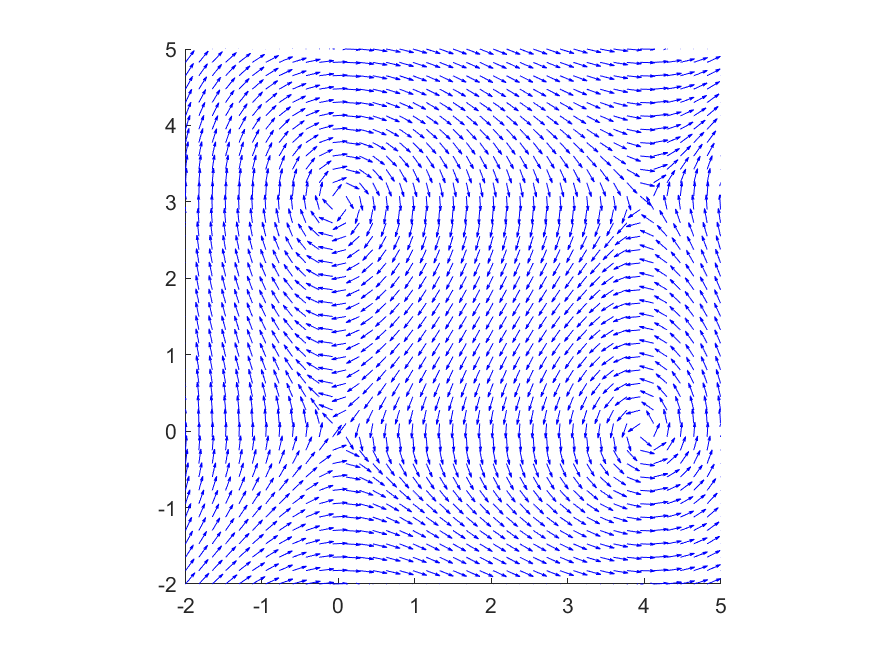
\includegraphics[width=0.6\textwidth]{../figures/NLVF_1.png}
    \end{center}
\end{exercise}
%\comboSol
%{%
%
%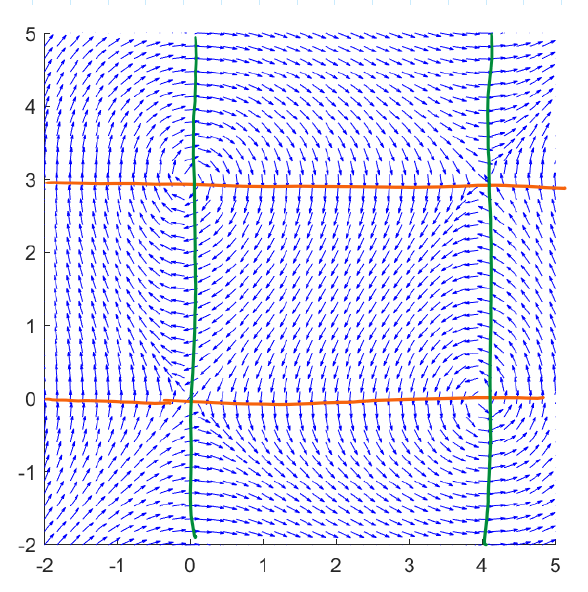
\includegraphics[width=1.5in]{Images/NLVF_1_Soln.png}
%}

\begin{exercise}
    Nullclines apply to linear systems as well, although since we can often solve those explicitly they're less necessary. Construct the nullcline diagram for the system $\dfrac{dx}{dt}=-3x+y$, $\dfrac{dy}{dt}=6x+2y$, and use it to classify (by type) the equilibrium point at the origin. 
    
    \wordChoice{\choice[correct]{center}\choice{saddle}}
    
    \begin{feedback}
        What is the {\it linearization} of this system at $(0,0)$?
    \end{feedback}
\end{exercise}
%\comboSol
%{%
%Saddle \hfill\raisebox{-0.5\height}{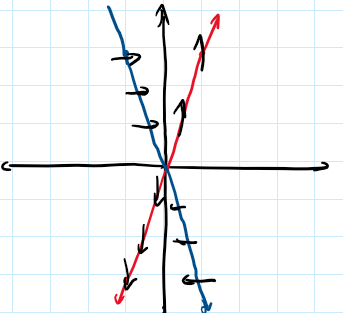
\includegraphics[height=1.2in]{Images/NullclineDiagramSoln1.png}}\hfill\hfill
%}

\begin{exercise}
    Consider the system $\displaystyle \frac{dx}{dt}= -2x+y, \frac{dy}{dt}=-y+x^2$.
    \begin{itemize}
        \item Find all equilibrium solutions. $\left(\answer{0}, \answer{0}\right)$, $\left(\answer{2}, \answer{4}\right)$
        \item Sketch all nullclines for this system on a single diagram. Label each region, and use these results to classify each equilibrium point.
    \end{itemize}
\end{exercise}
%\comboSol
%{%
%$(0,0)$ and $(2, 4)$. \hfill\raisebox{-0.5\height}{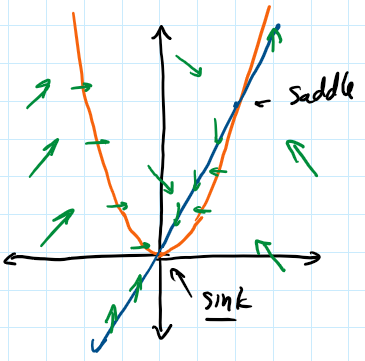
\includegraphics[height=1.2in]{Images/NullclineDiagramSoln2.png}}\hfill\hfill
%}

\begin{exercise} Nullclines need not be lines. Consider the system
    \[
        \begin{bmatrix} 
            \displaystyle \frac{dx}{dt}=4-y^2\\ 
            \dfrac{dy}{dt}=8-x^2-y^2 
        \end{bmatrix}.
    \]
    
    Find all critical points of this system: $\left(\answer{2}, \answer{2}\right)$, $\left(\answer{2}, \answer{-2}\right)$, $\left(\answer{-2}, \answer{2}\right)$, $\left(\answer{-2}, \answer{-2}\right)$
    \begin{problem}
        Classify (according to type) any critical point(s) that can be classified using nullcline analysis.\\
        $(2,2)$ is a \wordChoice{\choice{center}\choice[correct]{saddle}} \\
        $(-2, -2)$ is a \wordChoice{\choice{center}\choice[correct]{saddle}}.
        \begin{problem}
            Two critical points cannot be classified using the nullcline analysis. Classify these (again according to type) using the Jacobian. 
            $(-2, 2)$ is a \wordChoice{\choice{nodal}\choice[correct]{spiral}\choice{None of the other options}} \wordChoice{\choice{center}\choice{saddle}\choice[correct]{sink}\choice{source}} \\
            $(2, -2)$ is a  \wordChoice{\choice{nodal}\choice[correct]{spiral}\choice{None of the other options}} \wordChoice{\choice{center}\choice{saddle}\choice{sink}\choice[correct]{source}}. 
        \end{problem}
    \end{problem}
\end{exercise}
%\comboSol
%{%
%\begin{multicols}{2}
%\noindent a)~$(2, 2)$, $(2, -2)$, $(-2, 2)$, $(-2, -2)$ \quad b)~$(2,2)$ is a saddle, $(-2, -2)$ is a saddle. \quad c)~ $(-2, 2)$ is a spiral sink, $(2, -2)$ is a spiral source.
%
%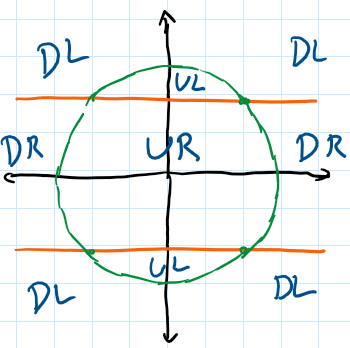
\includegraphics[height=1.2in]{Images/NullclineDiagramSoln3.png}
%\end{multicols}
%}

\begin{exercise}
    Consider the system
    \begin{equation}
        \begin{bmatrix}
            \frac{dx}{dt}=x-y^2+2\\[12pt]
            \frac{dy}{dt}=x^2-y^2
        \end{bmatrix}
        \label{eq:CriticalHamilEx}
    \end{equation}
    %5.1
    
    Find all critical points of \eqref{eq:CriticalHamilEx}.\\
        $\left(\answer{2}, \answer{2}\right)$, $\left(\answer{-1}, \answer{-1}\right)$, $\left(\answer{2}, \answer{-2}\right)$, $\left(\answer{-1}, \answer{1}\right)$
    \begin{problem}
        Create the nullcline diagram for the system, labelling each region as one of UL, UR, DL, or DR. Use this information to classify two critical points according to type.\\
        $(2, -2)$ is a \wordChoice{\choice{center}\choice[correct]{saddle}}. \\
        $(-1, 1)$ is a \wordChoice{\choice{center}\choice[correct]{saddle}}.
        \begin{problem}
            Use the Jacobian matrix to classify any remaining critical points.
            $(2, 2)$ is a \wordChoice{\choice{nodal}\choice[correct]{spiral}\choice{None of the other options}} \wordChoice{\choice{center}\choice{saddle}\choice[correct]{sink}\choice{source}}. \\
            $(-1, -1)$ is a \wordChoice{\choice{nodal}\choice[correct]{spiral}\choice{None of the other options}} \wordChoice{\choice{center}\choice{saddle}\choice{sink}\choice[correct]{source}}.
            \begin{problem}
                Is there a conserved quantity (Hamiltonian function) for this system?
                \begin{multipleChoice}
                    \choice{Yes.}
                    \choice[correct]{No.}
                \end{multipleChoice}
            \end{problem}
        \end{problem}
    \end{problem}
\end{exercise}
%\comboSol
%{%
%\begin{multicols}{2}
%\noindent a)~$(2, 2)$, $(-1, -1)$, $(2, -2)$, $(-1, 1)$ \quad b)~$(2, -2)$ is a saddle, $(-1, 1)$ is a saddle. \quad
%c)~$(2,2)$ is a spiral sink, $(-1, -1)$ is a spiral source. \quad d)~ No, can not have sources or sinks.
%
%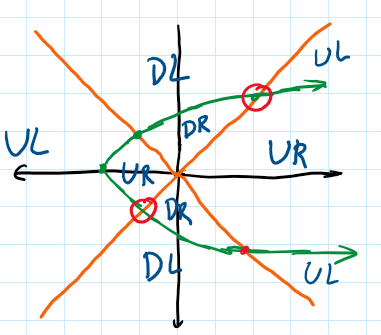
\includegraphics[height=1.2in]{Images/NullclineDiagramSoln4.png}
%\end{multicols}
%}

\begin{exercise}
    For a conflict between two armies, Lanchester's Law asserts that $\dfrac{dx}{dt}=-\alpha y$ and $\dfrac{dy}{dt}=-\beta x$, %5.2 (Hamiltonian, separatrix) 
    where $x$ and $y$ are the two populations, and $\alpha$ and $\beta$ are some positive constants.
    
    \begin{itemize}
        \item Find a Hamiltonian function for this system satisfying $H(0,0)=0$. $\answer{\beta\frac{x^2}{2} - \alpha \frac{y^2}{2}} = 0$
        \item Classify the critical point at the origin according to type {\bf and} stability. \wordChoice{\choice{center}\choice[correct]{saddle}}.
        \item Assume that we are just looking at the first quadrant, since the populations are non-negative. Find the curve along which the Hamiltonian function is zero, and explain its significance in terms of who wins the conflict.\\
        $y = \answer{\sqrt{\frac{\beta}{\alpha}}x}$
    \end{itemize}
\end{exercise}
%\comboSol
%{%
%a)~ $\beta\frac{x^2}{2} - \alpha \frac{y^2}{2} = 0$ \quad b)~Saddle, these are hyperbolas. \quad c)~ $y = \sqrt{\frac{\beta}{\alpha}}x$, dividing line deciding who wins
%}

\begin{exercise}
    Consider the non-linear system
    \begin{equation}
        \frac{dx}{dt}=4x-3y-x(x^2+y^2), \ \frac{dy}{dt}=3x+4y-y(x^2+y^2). \label{eq:NonLinStabLimitEx1} %5.1 or 2
    \end{equation}
    \begin{itemize}
        \item \eqref{eq:NonLinStabLimitEx1} has a critical point at the origin. What is the {\it linearization} of \eqref{eq:NonLinStabLimitEx1} at the origin?\\
            \wordChoice{\choice{nodal}\choice[correct]{spiral}\choice{None of the other options}} \wordChoice{\choice{center}\choice{saddle}\choice{sink}\choice[correct]{source}}
        \item Demonstrate that \eqref{eq:NonLinStabLimitEx1} is {\it locally linear} in a neighborhood of the origin. 
        \item Classify the origin according to its {\it type} and {\it stability}.\\
            \wordChoice{\choice{stable}\choice[correct]{unstable}} \wordChoice{\choice{nodal}\choice[correct]{spiral}\choice{None of the other options}} \wordChoice{\choice{center}\choice{saddle}\choice{sink}\choice[correct]{source}}
    \end{itemize}
\end{exercise}
%\comboSol
%{%
%a)~Spiral Source \quad b)~Matrix is invertible \quad c)~Unstable spiral source
%}

\begin{exercise} 
    Consider the system of differential equations
    \begin{equation}
        \frac{dx}{dt} = (x^2 - 1)y \qquad \frac{dy}{dt} = (y-3)(y-1)x \label{eq:NonLinBoAExam1}
    \end{equation}
    which has slope field sketched below.
    \begin{center}
        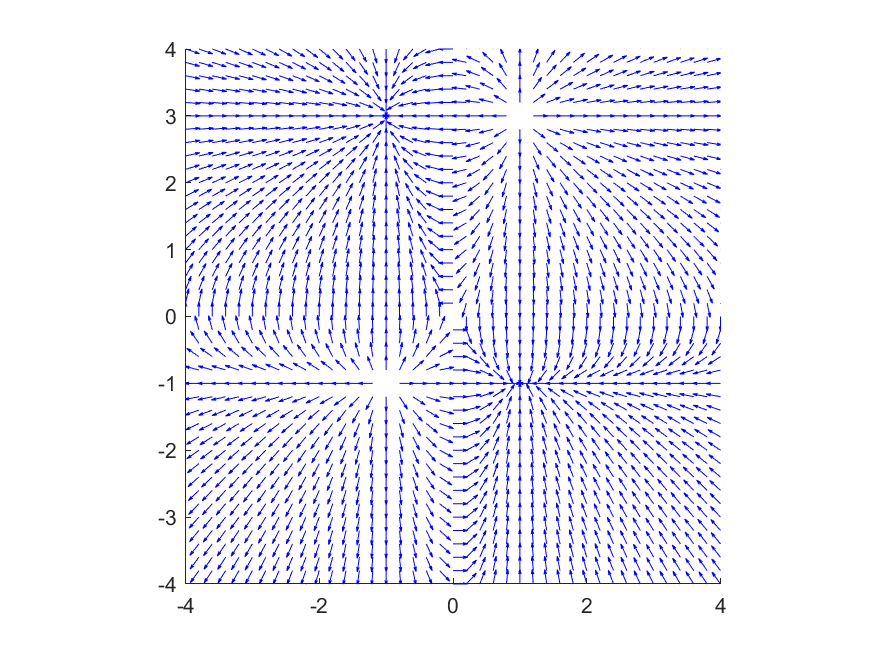
\includegraphics[width=0.6\textwidth]{../figures/NLBoA_Ex1.png}
    \end{center}
    \begin{itemize}
        \item Find and classify all critical points of the system \eqref{eq:NonLinBoAExam1}.
            $\left(\answer{-1}, \answer{-1}\right)$ \wordChoice{\choice[correct]{Nodal}\choice{spiral}\choice{None of the other options}} \wordChoice{\choice{center}\choice{saddle}\choice{sink}\choice[correct]{source}}. \\
            $\left(\answer{-1}, \answer{3}\right)$ \wordChoice{\choice[correct]{Nodal}\choice{spiral}\choice{None of the other options}} \wordChoice{\choice{center}\choice{saddle}\choice[correct]{sink}\choice{source}}. \\
            $\left(\answer{0}, \answer{0}\right)$ \wordChoice{\choice{Nodal}\choice{spiral}\choice[correct]{None of the other options}} \wordChoice{\choice{center}\choice[correct]{saddle}\choice{sink}\choice{source}}. \\
            $\left(\answer{1}, \answer{-1}\right)$ \wordChoice{\choice[correct]{Nodal}\choice{spiral}\choice{None of the other options}} \wordChoice{\choice{center}\choice{saddle}\choice[correct]{sink}\choice{source}}. \\
            $\left(\answer{1}, \answer{3}\right)$ \wordChoice{\choice[correct]{Nodal}\choice{spiral}\choice{None of the other options}} \wordChoice{\choice{center}\choice{saddle}\choice{sink}\choice[correct]{source}}. \\
        \item Draw any separatrices that you can spot on the slope field.
        \item Do any of these critical points have a basin of attraction? If so, sketch out what regions of the plane correspond to a basin of attraction for those critical points. 
    \end{itemize}
\end{exercise}
%\comboSol
%{%
%\begin{multicols}{2}
%\noindent $(1, -1)$ Nodal sink, $(-1, -1)$ Nodal source, $(1, 3)$ Nodal source, $(-1, 3)$ Nodal sink, $(0,0)$ Saddle. 
% \quad c)~ Yes, bottom right goes to $(-1, 1)$, top left goes to $(-1, 3)$.
% 
% 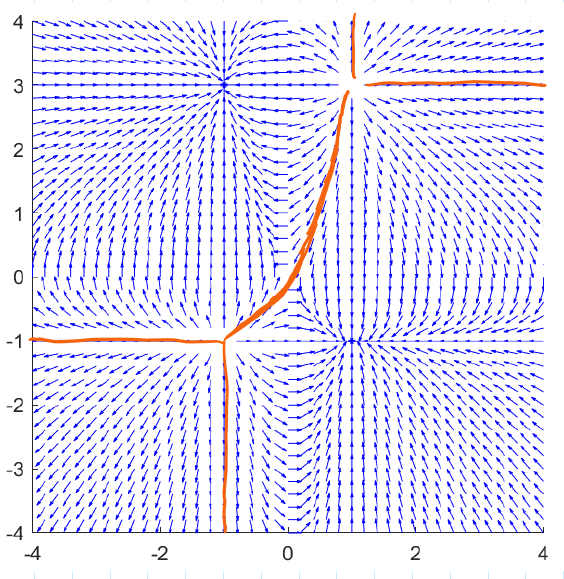
\includegraphics[width=1.2in]{Images/NLBoA_Ex1_Soln.png}
%\end{multicols}
%}

\begin{exercise} 
    Consider the system of differential equations
    \begin{equation}
        \frac{dx}{dt} = (2-y)(y+1)(x+1) \qquad \frac{dy}{dt} = -(x+2)(x-1)y \label{eq:NonLinBoAExam2}
    \end{equation}
    which has slope field sketched below.
    \begin{center}
        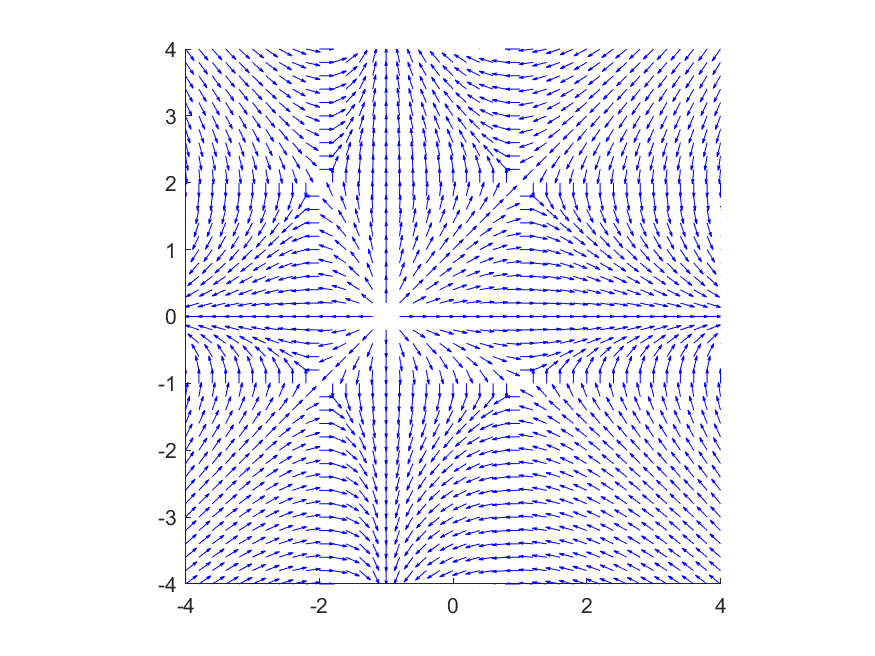
\includegraphics[width=0.6\textwidth]{../figures/NLBoA_Ex2.png}
    \end{center}
    \begin{itemize}
        \item Find and classify all critical points of the system \eqref{eq:NonLinBoAExam2}.\\
            $\left(\answer{-2}, \answer{-1}\right)$ \wordChoice{\choice{Nodal}\choice{spiral}\choice[correct]{None of the other options}} \wordChoice{\choice{center}\choice[correct]{saddle}\choice{sink}\choice{source}}. \\
            $\left(\answer{-2}, \answer{2}\right)$ \wordChoice{\choice{Nodal}\choice{spiral}\choice[correct]{None of the other options}} \wordChoice{\choice{center}\choice[correct]{saddle}\choice{sink}\choice{source}}. \\
            $\left(\answer{-1}, \answer{0}\right)$ \wordChoice{\choice[correct]{Nodal}\choice{spiral}\choice{None of the other options}} \wordChoice{\choice{center}\choice{saddle}\choice{sink}\choice[correct]{source}}. \\
            $\left(\answer{1}, \answer{-1}\right)$ \wordChoice{\choice{Nodal}\choice{spiral}\choice[correct]{None of the other options}} \wordChoice{\choice{center}\choice[correct]{saddle}\choice{sink}\choice{source}}. \\
            $\left(\answer{1}, \answer{2}\right)$ \wordChoice{\choice{Nodal}\choice{spiral}\choice[correct]{None of the other options}} \wordChoice{\choice{center}\choice[correct]{saddle}\choice{sink}\choice{source}}. \\
        \item Draw any separatrices that you can spot on the slope field.
        \item Do any of these critical points have a basin of attraction? If so, sketch out what regions of the plane correspond to a basin of attraction for those critical points. 
    \end{itemize}
\end{exercise}
%\comboSol
%{%
%\begin{multicols}{2}
%\noindent $(-2, 2)$ saddle, $(-2, -1)$ saddle, $(1, 2)$ saddle, $(1, -1)$ saddle, $(-1, 0)$ nodal source.
% \quad c)~ No.
% 
% 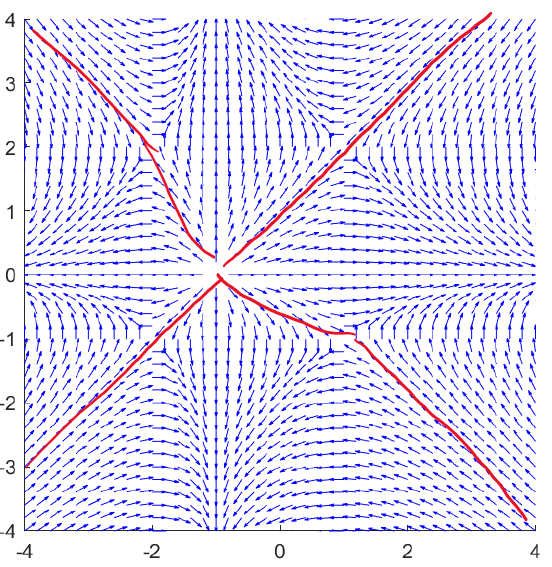
\includegraphics[width=1.2in]{Images/NLBoA_Ex2_Soln.png}
%\end{multicols}
%}


\end{document}